\documentclass{article}
\usepackage[utf8]{inputenc}
\usepackage{polski}

\usepackage{movie15}
\usepackage{amssymb, amsmath, amsfonts, amsthm, cite, mathtools, enumerate, rotating, hyperref, enumitem, graphicx, subfig,algorithmic,algorithm}
\newcommand \eq[1]{\begin{equation} \begin{split}  #1 \end{split} \end{equation}}
\graphicspath{ {../../wykresy/} }

\makeatletter
\newcommand\tab[1][1cm]{\hspace*{#1}}
\def\@seccntformat#1{%
  \expandafter\ifx\csname c@#1\endcsname\c@section\else
  \csname the#1\endcsname\quad
  \fi}
\makeatother

\title{Raport z projektu \textbf{Genetic Painting}}
\date{15.12.2021}
\author{Maurycy Borkowski}
\begin{document}
\maketitle
\section{Przedstawienie problemu}
Rozważamy problem \textit{malowania} istniejących już obrazów prostymi figurami geometrycznymi. To znaczy tworzenie kompozycji i dobór kolorów by całość przypominała zadany obraz. \href{https://rogerjohansson.blog/2008/12/07/genetic-programming-evolution-of-mona-lisa/}{Inspiracja} (i prawdopodobnie) autor problemu.\\\\
Jako podstawowego elementu kompozycji my użyjemy trójkąta.\\\\
Dokładniej, genotyp każdego osobnika będzie się składał z $k$ podstawowych elementów, trójkątów i ich kolorów. Fenotyp, trójkąt kodujemy za pomocą trzech par liczb, każda para odpowiada wierzchołkowi trójkąta, kolory kodujemy jako 4-krotki liczb z zakresu $[0,256]$, (RGBA).\\\\
Funkcja celu oblicza jakość osobnika w dwóch etapach:
\begin{itemize}
    \item Wygenerowanie obrazu (tablicy pixeli RGB) z danego osobnika
    \item Porównanie dwóch obrazów (MSE) i uśrednienie wyniku $\frac{1}{n \cdot m} \sum_i (p_i - o_i)^2$
\end{itemize}
\section{Rozwiązanie}
Okazuję się, że w rozwiązaniu tego problemu doskonale sprawdził prosty algorytm ewolucyjny:
\begin{algorithm}
\begin{algorithmic}
\STATE \textbf{input:} $N, T, N_d, obraz$
\STATE $P \leftarrow losowa\_populacja(N)$
\WHILE {$i \leq T$}
    \STATE {$P \leftarrow dodaj\_dzieci(N_d)$}
    \STATE {$P \leftarrow wybierz\_najlepsze(N, obraz)$}
    \STATE {$i \leftarrow i+1$}
\ENDWHILE
\RETURN $P_{max}$
\end{algorithmic}
\end{algorithm}
\\Dzieci dodajemy mutując każdego z osobników kilkukrotnie, z rozkładem normalnym zarówno współrzędne i kolory (o średniej w wartości rodzica). Z małym prawdopodobieństwem zmieniamy osobnika na losowego.\\
\section{Implementacja i pomysły}
Naiwne uruchomienie algorytmu od razu na pełnej przestrzeni poszukiwań kończyło się się niepowodzeniem, algorytm nie mógł znaleźć wzorca i ciągle błądził. Kluczem do sukcesu było dobieranie kilku trójkątów i \textit{mrożenie} poprzednich z najlepszego osobnika. W naszej implementacji dodajemy 1 trójkąt na 250 iteracji i zmieniamy tylko dwa najnowsze.\\\\
Dodatkowo by zwiększyć efektywność w implementacji zadbaliśmy by nie liczyć funkcji dopasowania (celu) dwa razy na tych samych osobnikach w każdej iteracji.\\\\
Początkowo algorytm i pomysły warto sprawdzać na małych rozmiarach obrazów, dla przyspieszenia obliczeń. Ostateczne obrazki liczą się $\approx 20$h.
\section{Wyniki}
Niestety z uwagi na bardzo długie obliczenia nie udało mi się zebrać wielu wyników i danych do analiz, ale o to część z nich.\\
Zgodnie z intuicją prostsze i mniejsze obrazy były o wiele łatwiejsze do przetworzenia.\\\\
Najlepsze obrazy powstały z populacji składającej się z jednego osobnika, co ciekawe jak widać na wykresie populacja pojedyńcza często długo dopasowywała świeżo dodany, losowy trójkąt. Mimo to ostateczne obrazy dla tych samych ilości wywołań funkcji celu powstawały z pojedyńczych populacji:
\begin{figure}[b!]
  \centering
  \subfloat[1 osobnik, 100 dzieci]{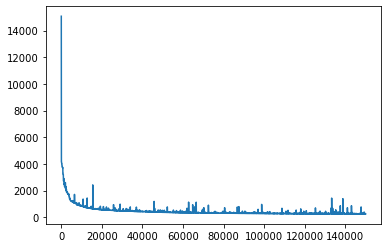
\includegraphics[width=0.5\textwidth]{static/wykres1}\label{fig:f1}}
  \hfill
  \subfloat[5 osobników, 20 dzieci]{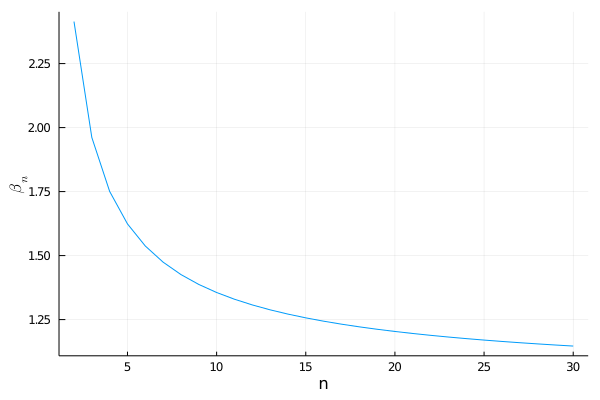
\includegraphics[width=0.5\textwidth]{static/wykres2}\label{fig:f2}}
\end{figure}
\\\\\\
\begin{figure}[t!]
  \centering
  \subfloat[1 osobnik, 100 dzieci]{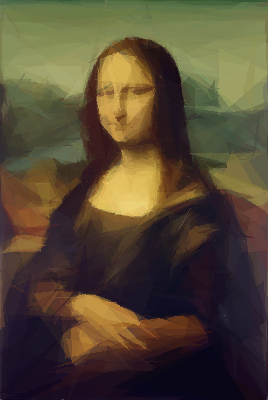
\includegraphics[width=0.5\textwidth]{results/150k1_100}\label{fig:f1}}
  \hfill
  \subfloat[5 osobników, 20 dzieci]{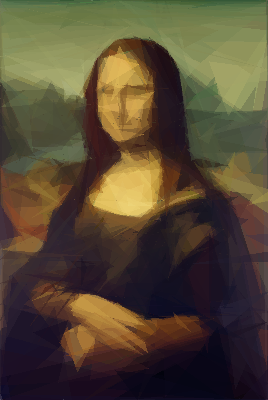
\includegraphics[width=0.5\textwidth]{results/150k5_20}\label{fig:f2}}
\end{figure}
Widać różnicę, zwłaszcza w szczegółach twarzy, przy tej samej liczbie trójkątów (600).\\\\
\\\\\\\\\\\\\\\\\\\\\\\\\\\\\\\\\\Niestety podobna ilość iteracji i trójkątów nie daje podobnie dobrych efektów bardziej skomplikowanym obrazom (mimo zbliżonych rozmiarów):
\begin{figure}[H]
  \centering
  \subfloat[wynik]{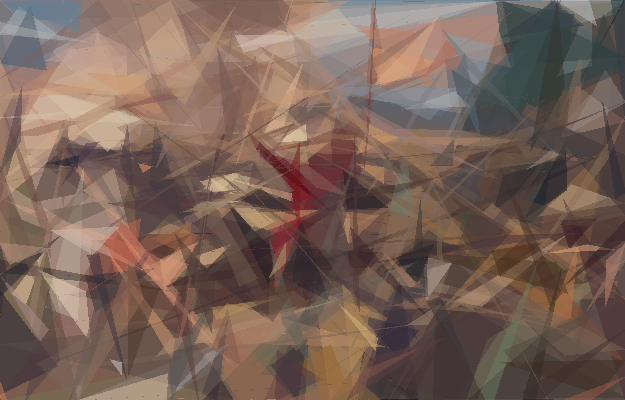
\includegraphics[width=1.0\textwidth]{results/Matejko100k}\label{fig:f1}}
  \hfill
  \subfloat[oryginał]{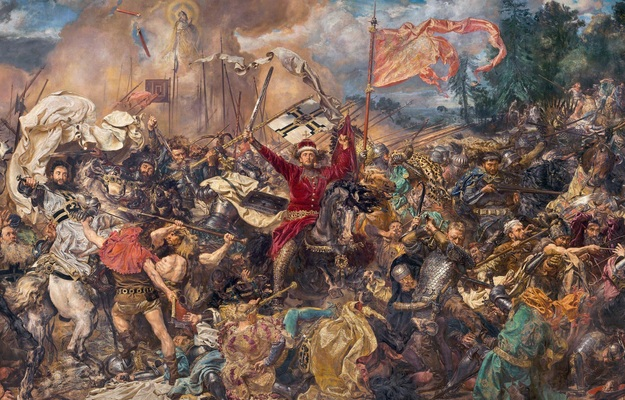
\includegraphics[width=1.0\textwidth]{static/matejko_medium}\label{fig:f2}}
\end{figure}
.\\\\\
Oto najlepsze dwa obrazy jakie udało mi się uzyskać przed kilkoma poprawkami:
\begin{figure}[H]
  \centering
  \subfloat[pierwszy dawałem trójkąty \textit{po kolei}]{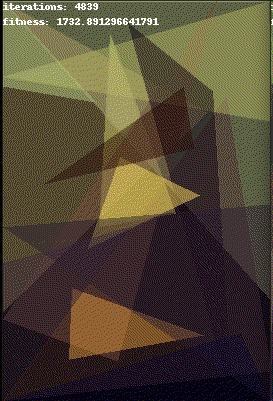
\includegraphics[width=0.5\textwidth]{results/sekwencyjna}\label{fig:f1}}
  \hfill
  \subfloat[pierwsze dłuższe obliczenia z tym pomysłem]{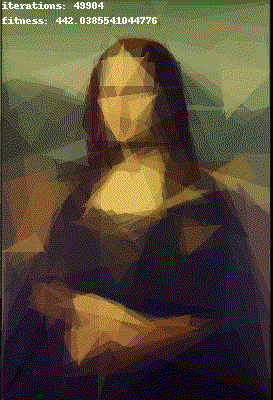
\includegraphics[width=0.5\textwidth]{results/firstnice}\label{fig:f2}}
\end{figure}
\section{Podsumowanie}
Zaskakująco trudne zadanie (do rozwiązania za pomocą standardowych metod) udało się rozwiązać dosyć prostym sposobem (i długimi obliczeniami). Wyniki są na prawde satysfakcjonujące, ciekawe jest obserwowanie przebiegu algorytmu, jak dobiera kolejne trójkąty (nagrania przebiegów iteracji są w plikach z wynikami).\\
Ten projekt był na prawdę ciekawy i przyjemny w realizacji, najważniejsza rzecz jakiej się nauczyłem, to żeby planować obliczenia i brać pod uwagę ich długość.

\end{document}